\documentclass[thesis.tex]{subfiles}

\title{Estimating duration in the presence of misclassification}
\author{Joshua Blake}
\date{\today}

\begin{document}

\ifSubfilesClassLoaded{
  \setcounter{chapter}{1}
}

\chapter{SARS-CoV-2: biology and data} \label{biology-data}

\todo[inline]{Rewrite chapter 2 intro after writing thesis intro because it will be clearer how to divide content.}

SARS-CoV-2 is a beta coronavirus that emerged in late 2019.
It is closely related to previous coronaviruses that have caused outbreaks in humans, SARS-CoV and MERS-CoV.

Coronaviruses are RNA (Ribonucleic acid) viruses.
RNA viruses use RNA, rather than DNA, as their genetic material.


\section{PCR testing} \label{biology-data:sec:PCR}

\todo[inline]{Consider finding or making a figure to explain PCR testing.}

PCR (Polymerase Chain Reaction) is a procedure that produces millions to billions of copies of a specific segment of DNA (Deoxyribonucleic acid) from a single copy~\autocite{smithPCR,garibyanPCR}.
This is known as \emph{amplifying} the DNA.
PCR has many uses within the biological sciences; Mark R.\ Hughes, deputy director of the Human Genome Project, has claimed it is the most important scientific technology of the last hundred years~\autocite{powledgePCR}.
It is central to the work in this thesis because it can be used to detect the presence of SARS-CoV-2 in a sample taken from a human, most commonly a nose and/or throat swab.

SARS-CoV-2 is an RNA virus, but PCR amplifies DNA.
Therefore, before the PCR process can be used to detect SARS-CoV-2, the RNA must be converted to DNA.
This process is known as \emph{reverse transcription}.
In reverse transcription, a naturally-occurring enzyme known as reverse transcriptase generates cDNA (complementary DNA) from the RNA in the sample~\autocites{valasekPower}.
Any sequence of cDNA has a one-to-one correspondence with a sequence of RNA.
The cDNA can then be used in the standard PCR process.

PCR consists of a series of cycles, each cycle containing a three-step process~\autocite{powledgePCR,garibyanPCR}.
The first step of the PCR cycle is \emph{denaturation}.
In denaturation, the DNA is heated to separate the two strands of DNA.
The second step is \emph{annealing}.
In annealing, the temperature is lowered to allow primers to bind to the DNA.
Primers are short sequences of DNA that are complementary to the DNA sequence of interest.
By choosing the primers, the PCR process targets a portion of DNA starting and ending with a specified sequence.
The final step is \emph{extension}.
In extension, the temperature is raised to allow the enzyme DNA polymerase to extend the primers and hence replicate the DNA sequence of interest.
In the course of such a cycle, the amount of DNA doubles.
Therefore, the number of DNA copies increases geometrically with the number of cycles completed.

Quantitative real-time (RT-)PCR gives a measurement of the amount of the target DNA sequence present in the original sample~\autocite{yangPCRdiagnostics}.
After each PCR cycle, the amount of target DNA is measured and compared to a pre-derived standard.
Once the measured amount of DNA exceeds the standard, the target DNA is said to be detected.
The number of cycles required to reach detection is known as the \emph{cycle threshold} (Ct) value.
Quantitative real-time PCR have a number of other practical advantages over previous PCR techniques (\eg speed); see \textcite{yangPCRdiagnostics,valasekPower} for more details.
All RT-PCR tests I consider in this thesis are quantitative real-time RT-PCR tests, and produce Ct values.

The Ct value decreases as the amount of DNA present in the original sample increases.
\todo{cite interpretation of Ct values}
If there is more RNA present, more DNA is created, and hence fewer cycles are required to reach detection.
The logarithm is because the process is geometric, and hence the number of DNA copies increases linearly on the log-scale each cycle.
Therefore, the Ct value is proportional to the negative log of the amount of DNA present in the original sample.
The amount of cDNA produced by reverse transcription is proportional to the amount of RNA present in the original sample.
Therefore, when testing for SARS-CoV-2, the Ct value is proportional to the negative log of the amount of SARS-CoV-2 RNA present in the original sample.

Like any diagnostic test, PCR tests are not perfect.
False positives and false negatives can occur.
These can be quantified in a number of ways.

The \emph{analytical sensitivity} of the test is the minimum number of copies of the target RNA material in the sample that the test can detect, typically expressed as the \emph{limit of detection}~\autocite{bustinMIQE}.
The limit of detection is the lowest concentration of the target RNA material that can be reliably detected using the procedure.
This is different to the \emph{clinical sensitivity} of the test, the ability of the test to detect a detectable individual (being detectable is defined in \cref{biology-data:sec:natural-history}).
Clinical sensitivity can be affected by a large variety of preanalytical factors, such as sample collection (\ie the swabbing process) and sample transportation~\autocite{lippiPotential}.
Clinical sensitivity is of primary interest in this thesis.
I will quantify it as the \emph{test sensitivity} (strictly the clinical test sensitivity), the probability of a positive test result for a detectable individual.
A negative result for a detectable individual is a \emph{false negative}.

The \emph{analytical specificity} of the test is the ability of the test to distinguish between the intended target rather than other, non-specific RNA (or DNA) sequences present in the sample~\autocite{bustinMIQE}.
As with sensitivity, this is different to the \emph{clinical specificity} of the test, the ability of the test to distinguish between detectable and undetectable individuals.
A positive result for an undetectable individual is a \emph{false positive}.
False positives are very rare for SARS-CoV-2 RT-PCR tests.
In summer 2020, the CIS performed 208,730 PCR tests and found only 159 positives, lower-bounding the test specificity (assuming all the positives are false positives) at 99.9\%~\autocite[section 5]{cisMethodsONS}.

RT-PCR enables the detection of SARS-CoV-2 viral RNA in a sample.
However, this does not necessarily mean that the virus is viable (\ie able to reproduce)~\autocite{puhachSARSCoV2}.
High viral loads (low Ct values) are more likely to be viable, but more sophisticated tests are required to determine viability.
The gold standard procedure is attempting to grow and recover viral material from a sample, a process known as \emph{cell culturing}~\autocite{singanayagamDuration,puhachSARSCoV2,hakkiOnset}.
Further details on cell culturing are beyond the scope of this thesis.

\section{Natural history of the disease} \label{biology-data:sec:natural-history}

\begin{figure}
  \makebox[\textwidth][c]{
  \begin{tikzpicture}[
      node distance = 4cm,
      on grid,
      auto,
      ->,>=stealth',
      every state/.style={draw,rectangle,align=center},
      ]

      \node[state] (pre) {RT-PCR negative \\ Not infectious};
      \node[state, right of=pre] (pos) {RT-PCR positive \\ Not infectious};
      \node[state, right of=pos] (infectious) {RT-PCR positive \\ Infectious};
      \node[state, right of=infectious] (not-infectious) {RT-PCR positive \\ Not infectious};
      \node[state, right of=not-infectious] (neg) {RT-PCR negative \\ Not infectious};

      \node[draw=none, below=2cm of pre] (infected) {} ;
      \node[draw=none, below=2cm of neg] (recovered) {} ;

      \node[above=2cm of pre] (titleA) {(A)};
      \node[below=1cm of infected] (titleB) {(B)};

      % \draw (0,-2) -- node {Infected} (pre);
      % \draw (not-infectious) -- (0,-2);

      \path (infected) edge node {Infected} (pre)
          (pre) edge (pos)
            (pos) edge (infectious)
            (infectious) edge (not-infectious)
            (not-infectious) edge (neg)
            (neg) edge (recovered);
    
    % Detectable
    \node[below = 1cm of infectious] (detect-label) {Detectable};
    \node[draw, thick, inner sep=0.3cm, fit=(pos) (infectious) (not-infectious) (detect-label), fill=blue!10,opacity=0.2] (detect-box) {};
  \end{tikzpicture}
  }
  \centering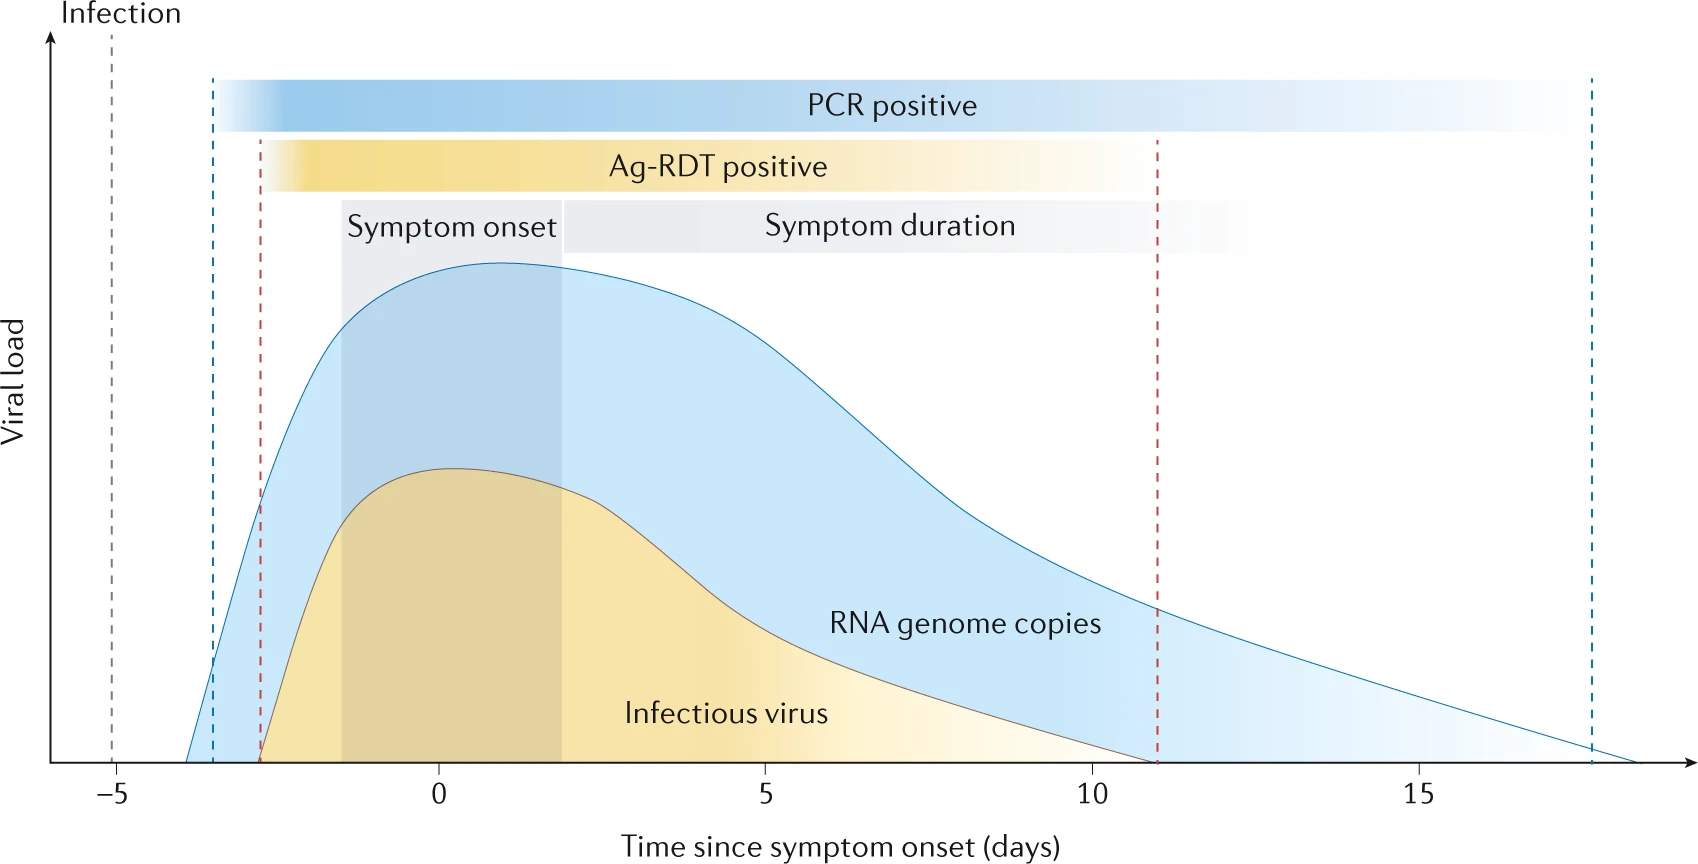
\includegraphics[width=\textwidth]{biology-data/natural-history}
  \caption[Natural history of SARS-CoV-2.]{%
    Natural history of SARS-CoV-2.
    (A) A simplified state-based model, which I generally use in this thesis.
    Shading represents states where the individual is detectable by a RT-PCR test.
    (B) A full model of the natural history, including continuous processes (Reproduced from \textcite{puhachSARSCoV2} with permission; durations are based on averages, there is a large amount of individual variation).
    PCR (strictly RT-PCR) positive refers to the main diagnostic test used in this thesis, and detect RNA genomes (see \cref{biology-data:sec:PCR} for more details).
    Ag-RDT (antigen rapid diagnostic test) tests are lateral flow tests, which detect infectious virus rather than RNA, and are not used in this thesis.
  }
  \label{biology-data:fig:natural-history}
\end{figure}

An individual infected with SARS-CoV-2 goes through several disease stages, depicted in \cref{biology-data:fig:natural-history}~\autocite{puhachSARSCoV2}.
First, they are exposed to the virus and become infected.
At this initial stage they are not infectious (cannot spread the disease to others), do not have symptoms, and will not test positive on a RT-PCR test.
After a few days, they will start testing positive on a RT-PCR test; this is normally prior to being infectious or having symptoms.
Next, the individual becomes infectious; normally, this occurs prior to symptom onset for those who experience symptoms.
Recovery from symptoms occurs after a few days, around the time the individual is no longer infectious.
Finally, the individual will test negative on a RT-PCR test.

The time for each of these stages depends on various features of host and virus characteristics.
In this thesis, I focus on pre-Alpha variants of SARS-CoV-2 in unvaccinated individuals.
The time from infection to infectiousness is known as the \emph{latent period}.
The length of the latent period is hard to estimate because neither the time of infection or the start of infectiousness can be observed; estimates for the mean length are generally 3--4 days~\autocite{zhaoEstimating}.
The time from infection to experiencing symptoms is known as the \emph{incubation period} and is estimated at have a mean length of around 6 days, with some sensitivity to the sampling and analysis technique used~\autocite{wuIncubation,quesadaIncubation,aleneSerial}.
The incubation period is undefined for asymptomatic individuals of those infected.

The above description gives three possible ways to define an individual who is infected with SARS-CoV-2: based on their RT-PCR test result, whether they are infectious, or whether they are symptomatic.
In this thesis, I adopt a definition of infection based on RT-PCR test results.
This is because it coincides with the data collected on the studies I use (see \cref{biology-data:sec:studies}).

A host's \emph{viral load}, the quantity of viral particles in a host, is the underlying biological process determining many of these changes~\autocite{puhachSARSCoV2}.
Any host's viral load is determined by the interaction of many biological processes, most prominently the virus's replication increasing the viral load and the host's immune response reducing the viral load~\autocite{keVivo}.
Viral replication requires the virus to infect a host cell and then use the host cell's machinery to produce more virus; as more host cells are infected this process slows because there are fewer remaining potential host cells, known as \emph{target cells}, to infect.
The host's immune system can slow this process by various mechanisms; the most relevant for SARS-CoV-2 is by making some target cells less susceptible to infection.
A host's immune response is triggered by the viral load, and becomes stronger as the viral load increases.
A high viral load is associated with being more infectious, more likely to test positive on a RT-PCR test, and the start of symptoms~\autocite{puhachSARSCoV2,keVivo}.


% Possible summaries
% \begin{enumerate}
%   \item \url{https://www.nature.com/articles/s41579-022-00822-w/figures/2}
%   \item \url{https://www.nature.com/articles/s41576-021-00360-w/figures/1}
%   \item \url{https://academic.oup.com/view-large/figure/305617142/ciaa1442_fig2.jpg}
% \end{enumerate}

\todo[inline]{Not sure if this is the best location for this important paragraph defining the concept of ``detectability''}
I will refer to individuals between the time they start testing positive on a RT-PCR test and the time they stop testing positive on a RT-PCR test as \emph{detectable}.
It is not possible to directly observe whether an individual is detectable or not due to noise in the RT-PCR test (see \cref{biology-data:sec:PCR}).
However, viewing the number of RNA genome copies in an individual as a latent process this can then be defined as the time when the number of RNA genome copies is above the limit of detection of the RT-PCR test.
While this definition is not perfectly precise, it is clear enough for the purposes it used in this thesis.



\section{Studies used in this thesis} \label{biology-data:sec:studies}

In this thesis, I use data from two studies which recruited participants from the general population in the UK.
Unlike many studies of SARS-CoV-2, these studies are not focused on specific groups such as healthcare workers or hospital patients.
Therefore, the results from these studies are more generalisable to the entire UK population.

\todo[inline]{Some of this might be moved into the introductory chapter motivating each part of the thesis.}

The first study, ATACCC (Assessment of Transmission and Contagiousness of COVID-19 in Contacts), performed daily testing of a small number of individuals with short follow-up.
The density of this sampling allows for reliable estimates of the viral load dynamics and other quantities of interest, most importantly the duration of detectability, but the results are limited because the small sample size and short follow-up means that the tails of these distributions cannot be estimated.

The second study, the CIS (Coronavirus (COVID-19) Infection Survey), performed weekly or monthly testing of a large number of individuals with long follow-up.
The large sample size and long follow-up allows for reliable estimates of the tails of the distributions of the quantities of interest.
However, the results are limited because the sparse sampling which means that the viral load dynamics cannot be estimated.
In particular, the vast majority of detected infections had only one or two positive tests, and hence the viral load trajectory of these infections cannot be estimated.

\subsection{Assessment of Transmission and Contagiousness of COVID-19 in Contacts}

The ATACCC study was a longitudinal study of contacts reported to the NHS Test and Trace contact tracing service~\autocite{hakkiOnset}.
Contacts were invited to participate if they were 5 years or older and  could be reached within 5 days of the index case's symptom onset date.
ATACCC was formed of two waves: ATACCC1 enrolled 393 contacts between 13th Sep 2020 and 31st Mar 2021 (when pre-Alpha and Alpha variants were circulating) and ATACCC2 enrolled 345 contacts between 24th May 2021 and 228th Oct 2021 (when the Delta variant was circulating).
Contacts were swabbed daily for up to 20 days, with a variety of tests performed on the swabs; relevant for this thesis is the RT-PCR test for SARS-CoV-2.
For all positive test results, the viral load was measured using the Ct value and then converted to a viral load using a standard curve.
Other data such as demography and symptoms was also collected.
For further details see \textcite{singanayagamDuration,hakkiOnset}.

\Textcite{hakkiOnset} analyse the viral load of the 57 contacts who tested positive for SARS-CoV-2 and had the growth phase in their viral load measured.
For 115 contacts with at least one positive RT-PCR test, the growth phase of viral load was not captured; these contacts were excluded from this analysis to ensure all individuals viral load trajectories could be identified.
I will revisit and extend this analysis in \cref{E-ATACCC}.

\subsection{Coronavirus (COVID-19) Infection Survey} \label{intro:sec:cis}

The CIS~\autocite{CIS} was setup in April 2020 to provide gold-standard measurements of the prevalence of SARS-CoV-2 in the community.
It is a longitudinal study with a representative sample of private households, this excludes settings such as care homes and student halls.
It is globally unique in providing a representative, longitudinal, and large-scale study.
Initially, it was limited to England, but expanded to cover the whole of the UK in September 2020.
Enrolment was continuous until 31st Jan 2022, with data collected until 13th Mar 2023~\autocite{weiRisk}. 

The CIS had a household-based design, meaning that households were invited to participate in the study.
From households that participated, all individuals aged 2 and over were invited to participate.
Once invited, an enrolment swab would be taken at the first visit followed by 4 further weekly visits (giving a total of 5 swabs on days 0, 7, 14, 21, 28 relative to enrolment) after which visits were monthly.
As well as a swab to test for SARS-CoV-2, participants were asked to complete a questionnaire, and some participants were asked to provide blood samples.
Real-world issues meant that visits were often not on this precise schedule, and occasionally missed.
A full description of the study can be found in the study protocol~\autocite{cisProtocol}.

Up until July 2020, households were selected from those that had previously participated in an ONS survey~\autocite{CIStechData}.
Around 50\% of households agreed to participate, with around 90\% of eligible individuals (96,113 in total) in these households contributing multiple swabs to the survey.
After July 2020, addresses were also randomly sampled from a database of all UK addresses held by the ONS.
The response rate was lower, with only 12\% of households agreeing to participate, from which 86\% of eligible individuals (383,732 in total) contributed multiple swabs to the survey.

These rates of response raise the possibility of non-response bias.
In particular, some demographic groups, such as young adults and individuals of non-white ethnicity, were underrepresented among those who responded~\autocite{pouwelsCommunity}.

In this thesis, I focus on the period from Mon 31st Aug 2020 until Sun 24th Jan 2021 (inclusive).
This period is chosen because there were very few positives in CIS in summer 2020 due to low prevalence and a smaller sample size, and ends when vaccination crossed 10\% of England's population.
Vaccination complicates the dynamics and immune response, which would require more complex models which are more specific to SARS-CoV-2 beyond the scope of this thesis, which primarily intends to show the potential of a study such as CIS in general.
\todo{make sure I justify the period choice in the intro when introducing the thesis's scope and aims}

During the start of this period, the recruitment rate of CIS was expanded (see \cref{biology-data:fig:CIS-recruitment}(A)).
Following this, the recruitment then decreases and stabilises, as does the rate of swabs taken (see \cref{biology-data:fig:CIS-recruitment}(B)).
The recruitment pattern was chosen to hit targets regarding the fortnightly number of swabs.
Because the testing becomes less frequent after the first 4 weeks, some continuous recruitment is needed to maintain the number of swabs, as well as to replace participants who drop out.

\begin{figure}
  \centering 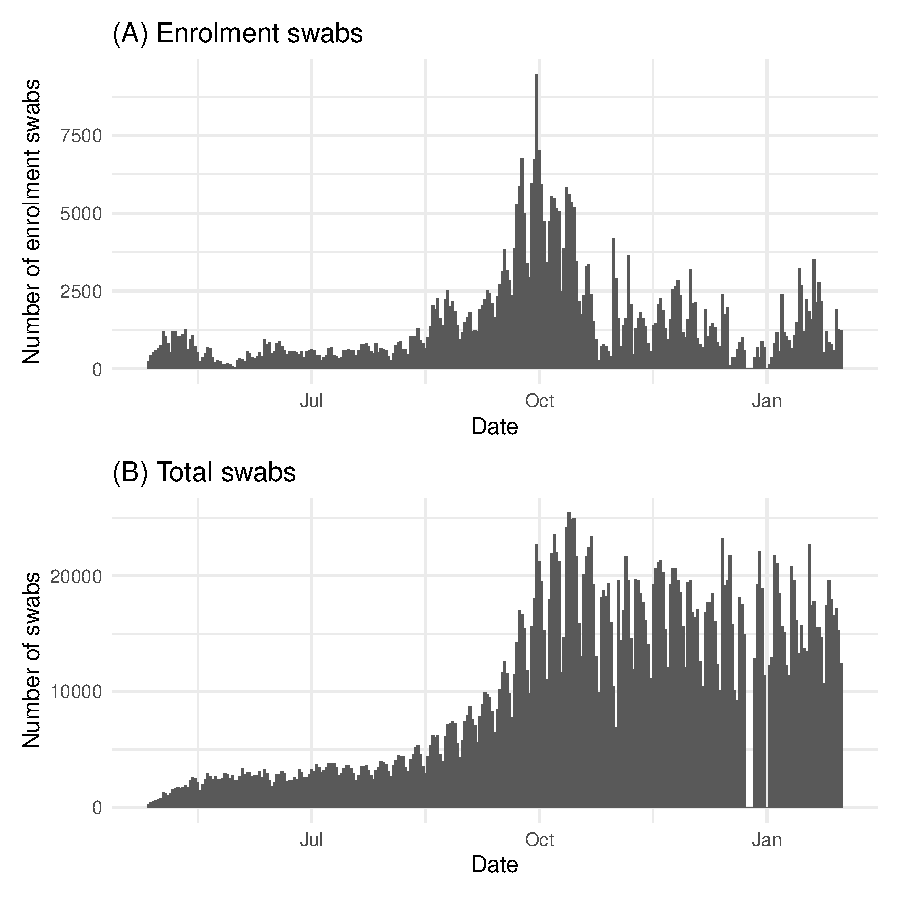
\includegraphics{biology-data/CIS-recruitment}
  \caption[CIS swab numbers]{%
    Number of swabs taken by the CIS in the period considered in this thesis (Sep 2020 until Jan 2021).
    (A) Only enrolment (\ie first) swabs for each individual.
    (B) Total swabs.
    Note the differing y-axis scales.
    Data from \textcite{CIStechData}.
  }
  \label{biology-data:fig:CIS-recruitment}
\end{figure}
% \begin{figure}
%   \centering 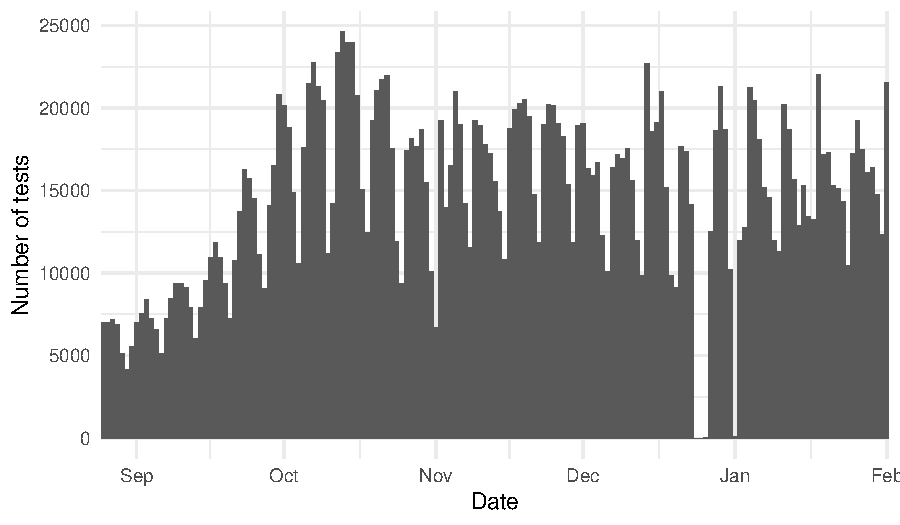
\includegraphics[width=\textwidth]{biology-data/CIS-num-tests}
%   \caption[Number of CIS tests]{%
%     Daily number of CIS tests conducted in the period considered in this thesis (Sep 2020 until Jan 2021).
%   }
%   \label{biology-data:fig:CIS-num-tests}
%   \todo[inline]{Cut this repetition of number of tests? Maybe highlight period of interest in previous plot}
% \end{figure}


\subsubsection{Estimating positivity rate}

The \emph{positivity rate} is the proportion of people in a given population that (if they were tested) would test positive for SARS-CoV-2 at a defined point in time; in this context test means an RT-PCR test~\autocite{cisMethodsONS}.
A notable feature of this definition is that it explicitly does not correct for false positive or negative results.
Generally, the point in time of interest is a specific day, although it has also been applied to a week~\autocite{cisMethodsONS,pouwelsMRPvaccination,pouwelsCommunity}.
Larger time periods (\ie weeks instead of days) allow more granular estimates in other dimensions, most commonly geography.

If the CIS was truly a random sample, an unbiased estimator of the positivity rate would be the proportion of positive tests in the sample; I refer to this as the uncorrected positivity rate.
However, in practice, two issues arise with this.
First, the non-response bias discussed previously.
Second, the number of positives on any day is low, especially among any specific subpopulation (\eg age group or region).
Statistical methods are used to correct for these issues.

The statistical preferred method for estimating the positivity rate is MRP (multi-level regression and poststratification)~\autocite{cisMethodsONS,pouwelsCommunity}.
The poststratification step is used to correct for non-response bias.
To address the low number of positives, MRP uses a hierarchical Bayesian model to borrow information across time and other covariates.
I explain the details of this model, and how I use it for estimating incidence in \cref{E-backcalc:sec:methods}

The outputs of this model compared to the raw positivity rate are shown in \cref{biology-data:fig:CIS-positivity}.
Both show similar trends.
The MRP estimate most often increases the estimated positivity rate, compared to uncorrected positivity rate, because the underrepresented demographic groups tended to have higher positivity rates.

\begin{figure}
  \centering 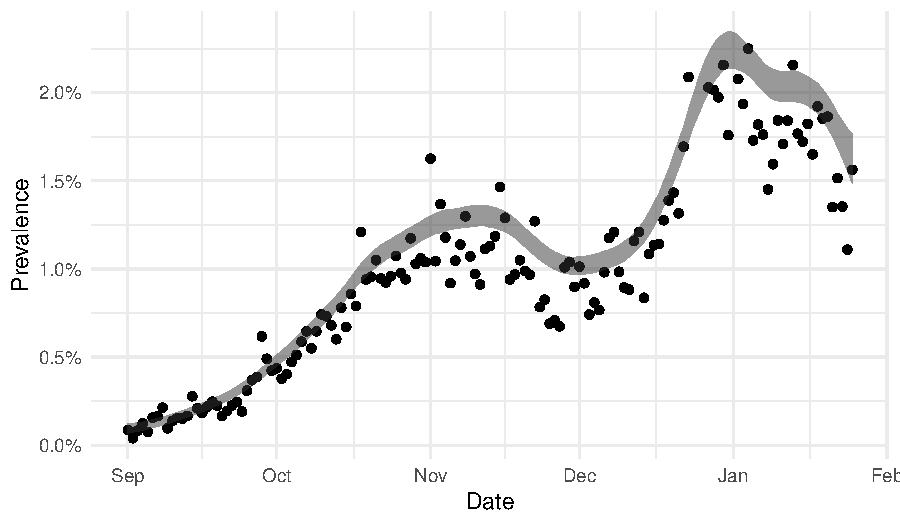
\includegraphics[width=\textwidth]{biology-data/CIS-positivity}
  \caption[CIS positivity]{%
    CIS positivity rate in the period considered in this thesis (Sep 2020 until Jan 2021).
    Dots show raw proportion of non-void tests that are positive on each day (days with fewer than 100 tests excluded for readability).
    Ribbon shows modelled 95\% CrI for the positivity, corrected for non-response bias and smoothed over time (using the methodology described in \cref{E-backcalc:sec:methods}).
  }
  \label{biology-data:fig:CIS-positivity}
\end{figure}

Interpreting positivity, or prevalence, directly is difficult because it is a delayed and smoothed measure of incidence (see \cref{E-inc-prev:sec:prevalence-process}).
The major aim of this thesis is the ability to produce estimates of incidence, which can be interpreted in terms of population behaviour.

As well as estimating the positivity rate for the whole of England (and the devolved nations), the CIS also estimates the positivity rate for various subpopulations, in particular geographic areas and age groups.
The exact specification of these have varied over time.

The geographic areas I will adopt are the nine standard regions of England (International Territorial Level 1, previously Nomenclature of Territorial Units for Statistics 1); these are: North East, North West, Yorkshire and the Humber (commonly abbreviated to Yorkshire), East Midlands, West Midlands, East, London, South East, and South West~\autoref{onsRegions}.
These are the geographic areas used throughout the major CIS analyses in England, although sometimes more granular areas were defined~\autocite[e.g.][]{pouwelsMRPvaccination,pouwelsCommunity,cisMethodsONS,houseInferring,walkerTracking}.

The age groups used have varied slightly for different CIS analyses~\autocite[e.g.][]{pouwelsMRPvaccination,pouwelsCommunity,cisMethodsONS,houseInferring,walkerTracking}.
I will use the age groups: 0--10 (pre-school and primary school), 11--15 (compulsory secondary school), 16--24 (adolescents and young adults who may remain in formal education), 25--49 (younger working age adults), 50--69 (older working age adults), and 70+ (elderly).

The household-based design of the CIS means that the data is clustered.
In particular, individuals in the same household are likely to transmit to each other and hence have correlated test results.
Other behavioural or genetic factors could also contribute to individuals in the same household being more similar than randomly selected individuals in the population.
The positivity analyses use a beta-binomial likelihood (defined in \cref{E-distributions}) to account for this.

The beta-binomial distribution is overdispersed relative to the binomial distribution.
Overdispersion allows for household clustering\todo{cite beta-binomial as a model for clustering} and other overdispersion in the data, which is common in epidemiological data\todo{cite that epi data is often overdispersed}. 
The parameterisation of the beta-binomial that I use (detailed in \cref{E-distributions}) has an overdispersion parameter $\rho$, regarded as a nuisance parameter in this context.
$\rho=0$ means the beta-binomial coincides with the binomial distribution.
As $\rho \to \infty$, the distribution tends towards the uniform distribution on $[0, 1]$~\autocite{hughesUsing}.

\subsubsection{Episodes}

Positive test results need to be grouped into \emph{infection episodes}.
An infection episode is a series of positive tests that originate from a single transmission event.
I use a heuristic-based algorithm developed throughout the pandemic, and published within \textcite{weiRisk}; see that publication for full justification of the criteria.

The algorithm determines whether a new positive tests, at time $t$, is part of the previous infection episode in the same individual, where that previous infection episode had its first positive test at $t_p$.
If the individual has no previous positive tests, the new positive test is always the start of a new infection episode.
Otherwise, the test at $t$, in the pre-Omicron era (prior to December 2021), is defined as the start of a new infection episode if any of the following apply.
\begin{enumerate}
  \item $n \geq 1$ and $t - t_p > 120$.
  \item $n \geq 2$ and $t - t_p > 90$.
  \item $n \geq 3$ and $t - t_p > 60$.
  \item $n \geq 4$.
  \item A complex heuristic based on the likely variant of the positive tests (see \textcite{weiRisk} for details). This heuristic rarely applied in the pre-Omicron era~\citePersonalComms{Sarah Walker}.
\end{enumerate}

A negative between two positive tests, when those positives are classed as part of the same infection episode, is known as an \emph{intermittent negative}.
Intermittent negatives are the clearest example of a false negative.
I will generally consider that intermittent negatives are uninformative on the duration of detectability, and hence exclude them from several analyses.

A sample of 500 randomly selected infection episodes (selected from the episodes used in the analyses in this thesis) have their test results shown in \cref{biology-data:fig:episodes}.
As can be seen, the number of tests within an episode, their length, and other characteristics vary greatly.
\begin{figure}
  \thisfloatpagestyle{empty}
  \vspace{-5cm}
  \makebox[\textwidth][c]{
\includegraphics[height=.7\paperheight]{biology-data/STATS13734/data_viz}}
  \caption[CIS infection episodes]{%
    500 randomly selected infection episodes.
    Shown are the negative tests before and after the outermost positive tests associated with the episode.
    Red dots are negative tests, green dots are positive tests, and blue dots are void tests (where the result could not be determined; excluded from other analyses).

    This figure has been provided as management information for operational planning purposes. They are provisional estimates circulated before public release. This management information should not be shared widely and should only be used for operational planning purposes. This information is not to be used publicly and ahead of being released publicly by ONS.
  }
  \label{biology-data:fig:episodes}
\end{figure}
  \todo{Work out what to do with this figure....}


\ifSubfilesClassLoaded{
  \listoftodos
}{}

\end{document}